\chapter{Project Management} \label{chap:project-management}
\section{Initial Project Plan}
The initial project plan can be seen below in \autoref{fig:initial_project_plan}. However, unfortunately
due to work commitments as well as other personal issues, the author was unable to keep to the initial plan.
The overall design of the plan remained constant, but the dates would be shifted and squeezed to the later dates.

\begin{figure}
    \centering
    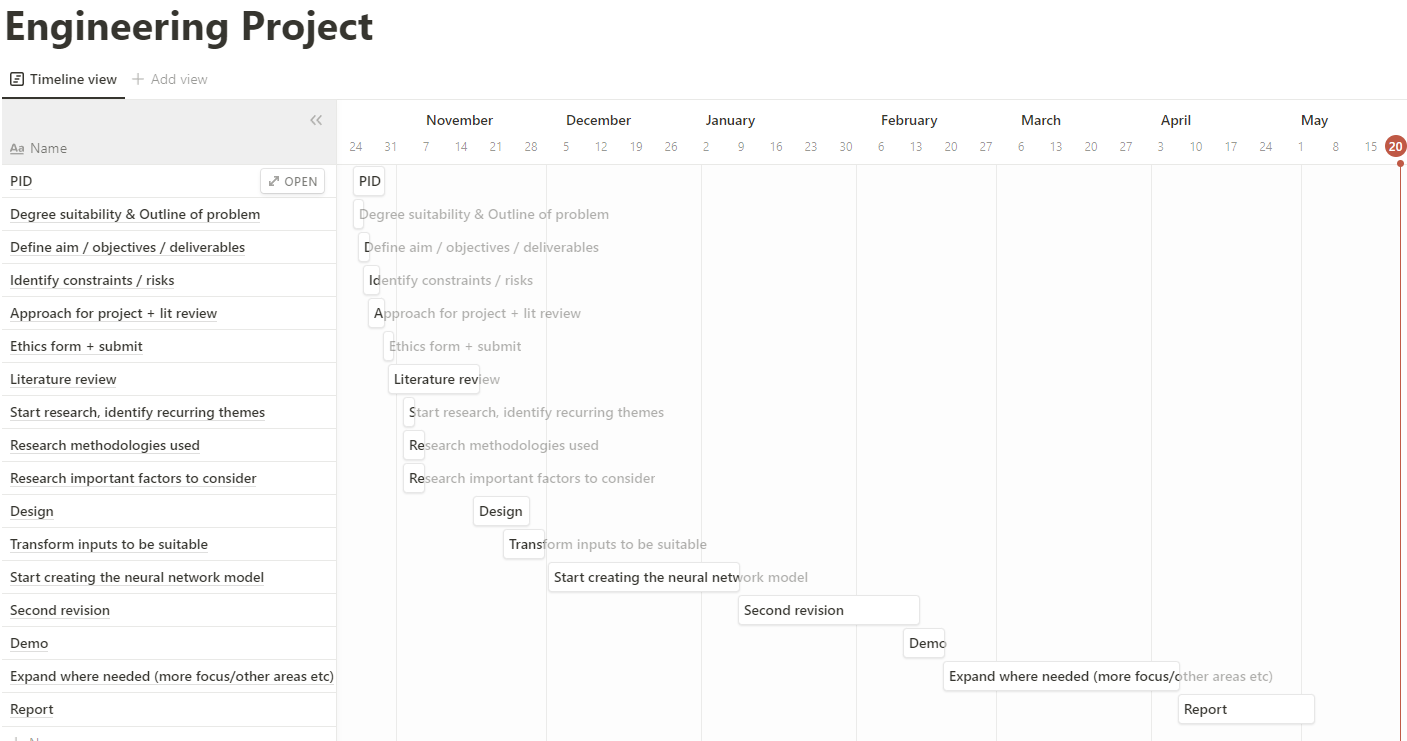
\includegraphics[width=0.95\columnwidth]{figures/initial_plan.png}
    \caption{A Gantt chart of the initial project plan}
    \label{fig:initial_project_plan}
\end{figure}
\FloatBarrier

\section{Version Control}
For version control of the project's code, Git was utilised as well as GitHub to be used as a backup
in case of any local device failures. Code was regularly committed as changes were made. The repository
containing the code, also contained the source material for the LaTeX document and as such any changes
to the project document were tracked in a similar manner.

The commit history between 13th March and 15th May can be seen in figure \autoref{fig:project_commit_history}.

\begin{figure}
    \centering
    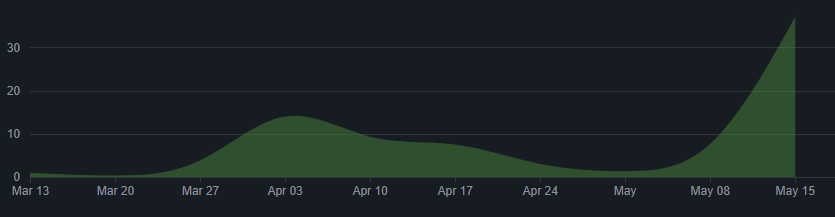
\includegraphics[width=0.95\columnwidth]{figures/commit_history.png}
    \caption{A chart of the commit history of the project}
    \label{fig:project_commit_history}
\end{figure}
\FloatBarrier
